%%%%%%%%%%%%%%%%%%%%%%%%%%%%%%%%%%%%%%%%%%%%%%%%%%%%%%%%%%%%%%%%%%%%%%%%%%
% Voltage U_um Section 
%%%%%%%%%%%%%%%%%%%%%%%%%%%%%%%%%%%%%%%%%%%%%%%%%%%%%%%%%%%%%%%%%%%%%%%%%%

\begin{solutionfigure}[ht]
    \centering
    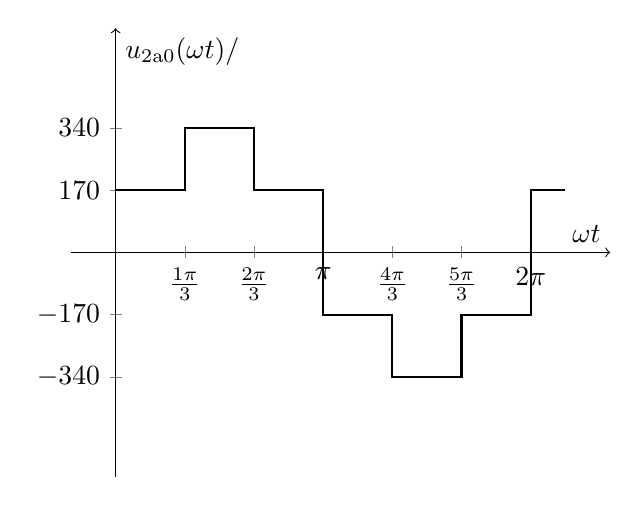
\begin{tikzpicture}
        \begin{axis}[
          %  width=7cm, height=5cm,
            axis lines=middle, 
            enlargelimits,
            axis line style={->}, % Pfeilspitzen an den Achsen
            xlabel={$\omega t$}, 
            ylabel={$u_\mathrm{2a0}(\omega t)/ \SI{}{\volt}$}, 
            xmin=0, xmax=13/6*pi,
            ymin=-1, ymax=1,
            xtick={0,  pi/3, 2*pi/3, pi, 4*pi/3, 5*pi/3, 2*pi},
            xticklabels={0, $\frac{1\pi}{3}$, $\frac{2\pi}{3}$,$\pi$, $\frac{4\pi}{3}$, $\frac{5\pi}{3}$, $2\pi$},
            ytick={-2/3, -1/3, 0, 1/3, 2/3},
            yticklabels={$-340$, $-170$, $0$, $170$, $340$},
          %  grid=both,
          %  major grid style={line width=.2pt,draw=gray!50},
          %  minor grid style={line width=.1pt,draw=gray!20},
        ]
                \addplot[
            thick,
            mark=none,
            color=black,
        ] coordinates {
          (0,1/3)  (1/3*pi, 1/3) (1/3*pi, 2/3)( 2/3*pi, 2/3) (2/3*pi, 1/3) (pi, 1/3) (pi, -1/3) (4/3*pi, -1/3) (4/3*pi, -1/3) (4/3*pi, -2/3) (5/3*pi, -2/3) (5/3*pi, -1/3) (2*pi, -1/3)  (2*pi, 1/3) (13/6*pi, 1/3)
        };
        \end{axis}
    \end{tikzpicture}
    \caption{Section of the voltage curve $u_\mathrm{2a0}(\mathrm{\omega t})$.}
    \label{fig:voltage_u2a0_section}
\end{solutionfigure}
